% Design & Architektur
% @author Tristan Ropers
%
\chapter{Design \& Architektur}

Zur Umsetzung der Anforderungen wurde eine RPC-Architektur entwickelt, die es ermöglicht den Prozess
abzubilden. Im folgenden Kapitel wird diese Architektur vorgestellt sowie ihre Besonderheiten.

\section{Systemkontext}

\begin{figure}[h]
 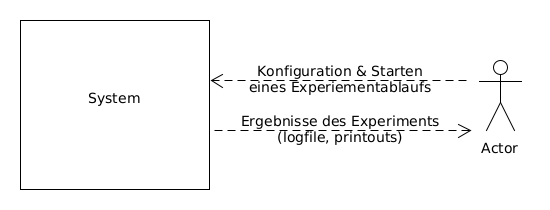
\includegraphics[width=\textwidth]{../diagrams/1_systemkontext.png}
 \caption{Systemkontext}
 \label{fig:systemkontext}
\end{figure}

Der Systemkontext des Gesamtsystems, wie in \ref{fig:systemkontext} zu sehen,
umfasst den Nutzer, welcher gleichzeitig Administrator ist und das Gesamtsystem.
Der Nutzer konfiguriert das System und startet im Anschluss die zuvor konfigurierte Konfiguration.
\clearpage

\section{Lösungsansatz}
\label{loesungsansatz}

Das System besteht aus einer RPC-Architektur und einer Robotersimulation. Die RPC-Architektur ermöglicht
die Kommunikation und Steuerung der Abläufe der Roboter untereinander und dient damit als Basis der
Architektur. Alle Nodes laufen auf einem Rechner, laufen also jeder auf einem Port.
Um den Bereich abzustecken, in dem die Nodes laufen wird in der Konfiugration ein Portbereich mitgegeben.
Dieser Bereich dient auch der Kommunikation der Roboter. Über den Portbereich lassen sich Nachrichten
als Broadcast an jeden Port verschicken.
Die Software wurde in der Programmiersprache \glqq Kotlin\grqq{} implementiert 
(\url{https://kotlinlang.org/}), die auf Java basiert. Als Entwicklungsumgebung wurde
IntellijIDEA Community 2020.3 (\url{https://www.jetbrains.com/idea/}) verwendet.

\subsection{Registrierung eines Roboters}

Die Roboter registrieren sich gegenseitig wenn das System hochgefahren wird. Sobald eine Node hochgefahren
wird, wird ein Broadcast auf dem Portbereich getätigt, damit wird jeder Roboter mit jedem bekanntgemacht
bevor die Wahl des Koordinators und Bestimmung des Zyklus losgeht. Somit hat man eine vollvermaschte
Peer-To-Peer Topologie.

\subsection{Bestimmung eines Zyklus}

Da die Nodes im System unabhängig von einer zentralen Einheit (bis auf Erhebung von Experimentdaten)
in einem Peer-To-Peer \citep{tanenbaumvansteen} Verbund existieren, muss zur Bestimmtung 
eines Zyklus eine Node die Rolle des Koordinators \citep{tanenbaumvansteen} übernehmen, welcher den Zyklus bestimmmt.\\
Zur Bestimmung des Koordinators wird zu Beginn des Experiments der Bully-Algorithmus \citep{tanenbaumvansteen}
als Wahlalgorithmus verwendet, bei diesem wird über die ID der Roboter bestimmt wer als
Koordinator gewählt wird.

\subsection{Schweißvorgang (Welding)}

Um den Schweißvorgang selbst zu simulieren wird beim welding() call in einer Node ein Thread gestartet,
der eine konfigurierte Zeit wartet um die mechanische Bewegung und das Schweißen der Roboter zu simulieren. Zusätzlich wird über die Konsole sowie in der Log-Datei eine Nachricht ausgegeben,
welche auf den Schweißvorgang hinweist.

\subsection{Logging der Prozessabläufe}

Um das Logging der verschiedenen Abläufe und Zustände sicherzustellen wurde ein Logging-Server implementiert,
der selbst über eine RPC Schnittstelle verfügt, auf dieser Log-Nachrichten der einzelnen Nodes übertragen
werden können.

\section{Architektur}

\subsection{Gesamtsystem}

\begin{figure}[h]
 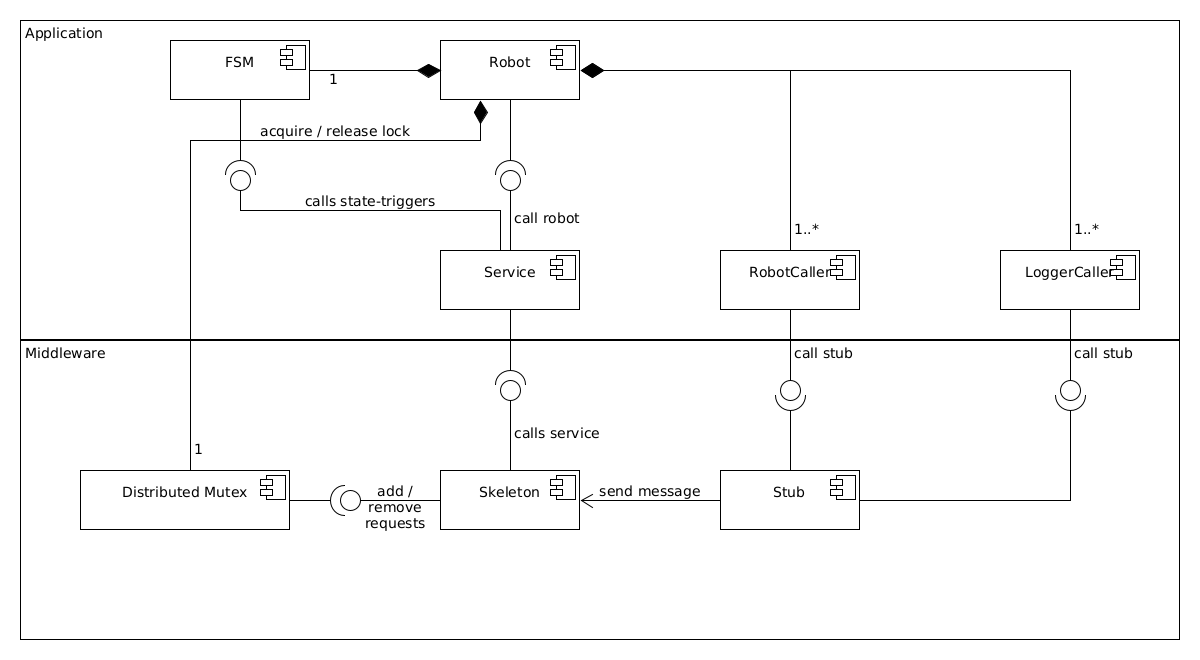
\includegraphics[width=\textwidth]{../diagrams/2_gesamtsystem.png}
 \caption{Komponentendiagramm Gesamtsystem}
 \label{fig:gesamtsystem}
\end{figure}

\clearpage

\subsection{Robot}

Eine zentrale Rolle in der Architektur spielt der Roboter, er beinhaltet Kommunikationselemente (Stubs 
\citep{tanenbaumvansteen} zu den anderen Robotern), eine Statemachine, eine Simulation des
Schweißvorgangs (siehe \ref{fig:gesamtsystem}) und eine Implementierung des verteilten gegenseitigen
Ausschluss (Distributed Mutex \ref{fig:gesamtsystem}).

\begin{figure}[h]
 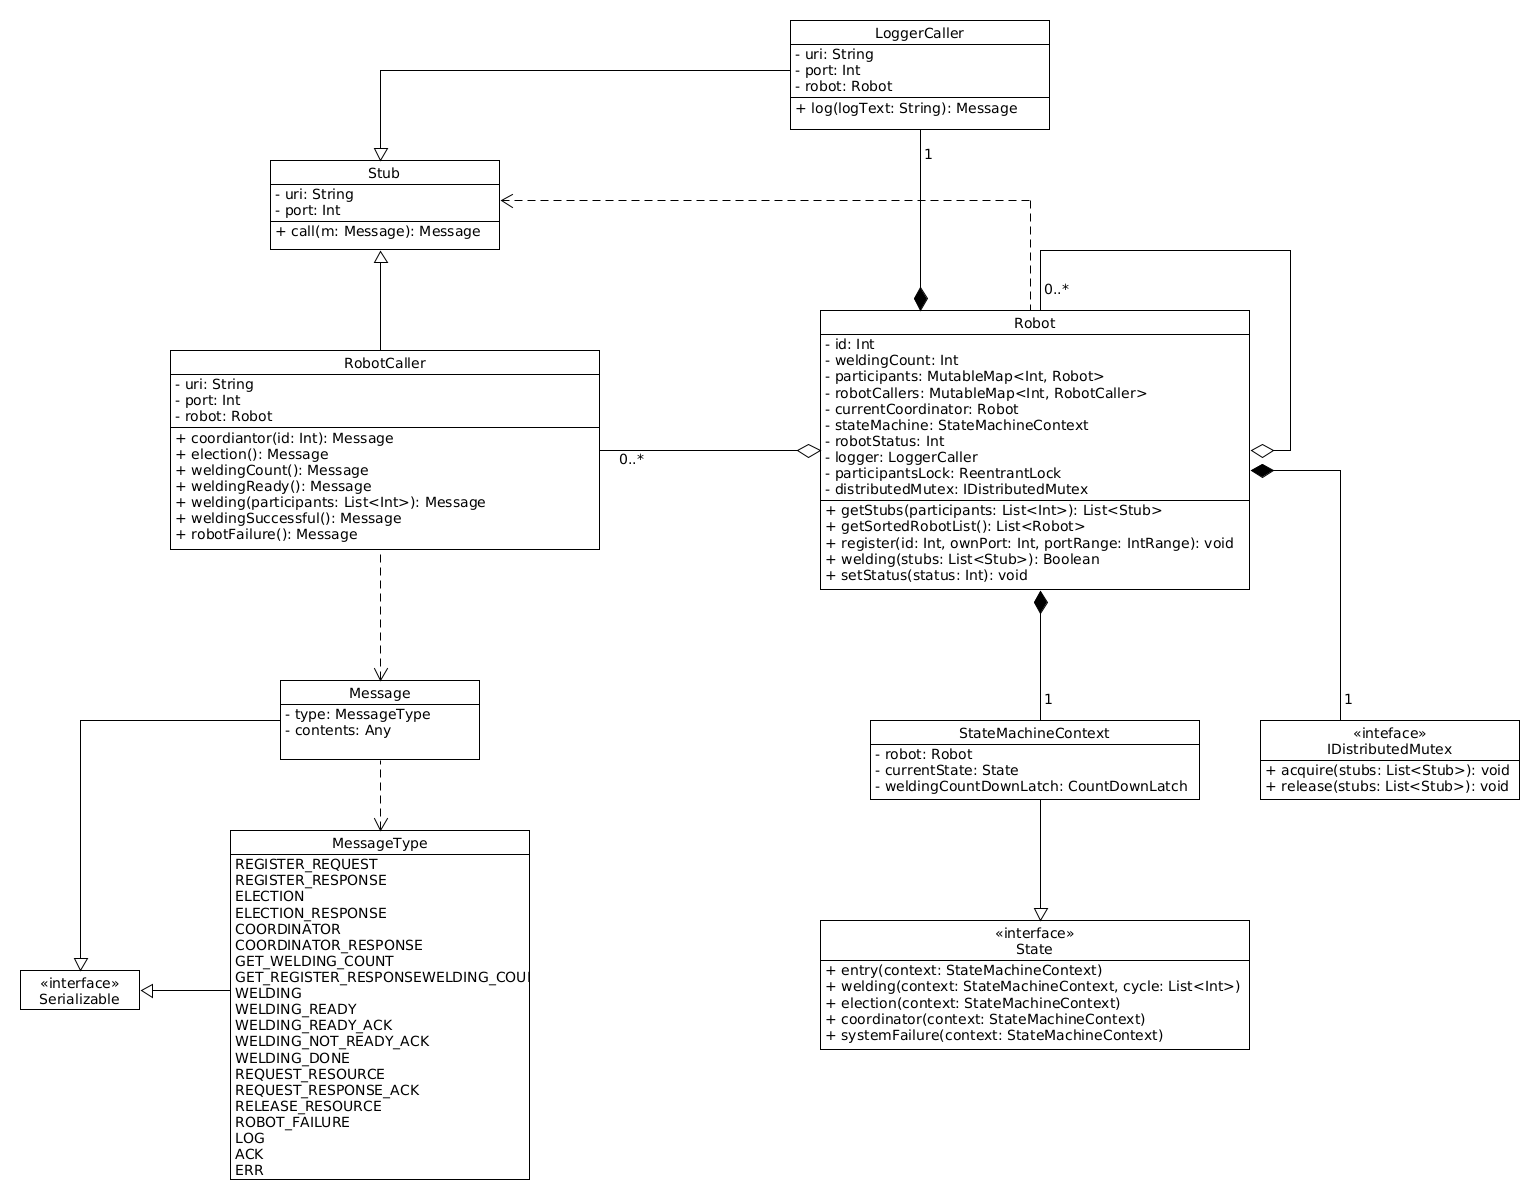
\includegraphics[width=\textwidth]{../diagrams/3_robot_klassendiagramm.png}
 \caption{Klassendiagramm Robot}
 \label{fig:class_robot}
\end{figure}

Im Klassendiagramm \ref{fig:class_robot} zu sehen ist die Implementierung der Robot-Klasse.
Wie vorher erwähnt sieht man hier die Bündelung der Funktionalitäten wie eine 
Instanz der FSM (StateMachineContext), die Robot- und LoggerCaller und den IDistributedMutex für
den verteilten gegenseitigen Ausschluss.

\clearpage

\subsection{Distributed Mutex}

\begin{figure}[h]
 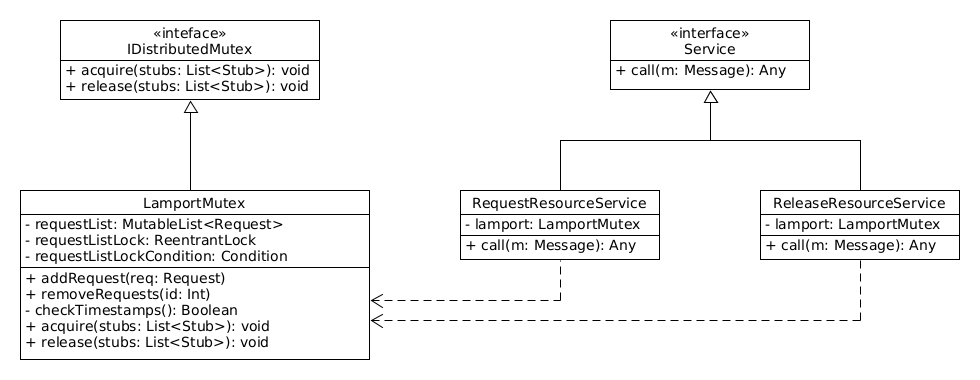
\includegraphics[width=\textwidth]{../diagrams/4_lamport_klassendiagramm.png}
 \caption{Klassendiagramm LamportMutex}
 \label{fig:class_lamport}
\end{figure}

In \ref{fig:class_lamport} zu sehen ist das Klassendiagramm des LamportMutex, der den Lamport-Algorithmus
implementiert. Damit die Austauschbarkeit des verwendeten Algorithmus (siehe \ref{table:reqmutexexchangable})
sichergestellt ist, wird das IDistributedMutex als Interface definiert und wie in \ref{fig:class_robot}
zu sehen im Robot mit der Implementierung des LamportMutex instanziiert. Die beiden Services RequestResourceService
und ReleaseResourceService sind Bestandteile der RPC-Architektur, über diese andere Roboter die Ressource
akquirieren (RequestResourceService) oder freigeben (ReleaseResourceService) können.

\clearpage

\subsection{FSM}

\begin{figure}[h]
 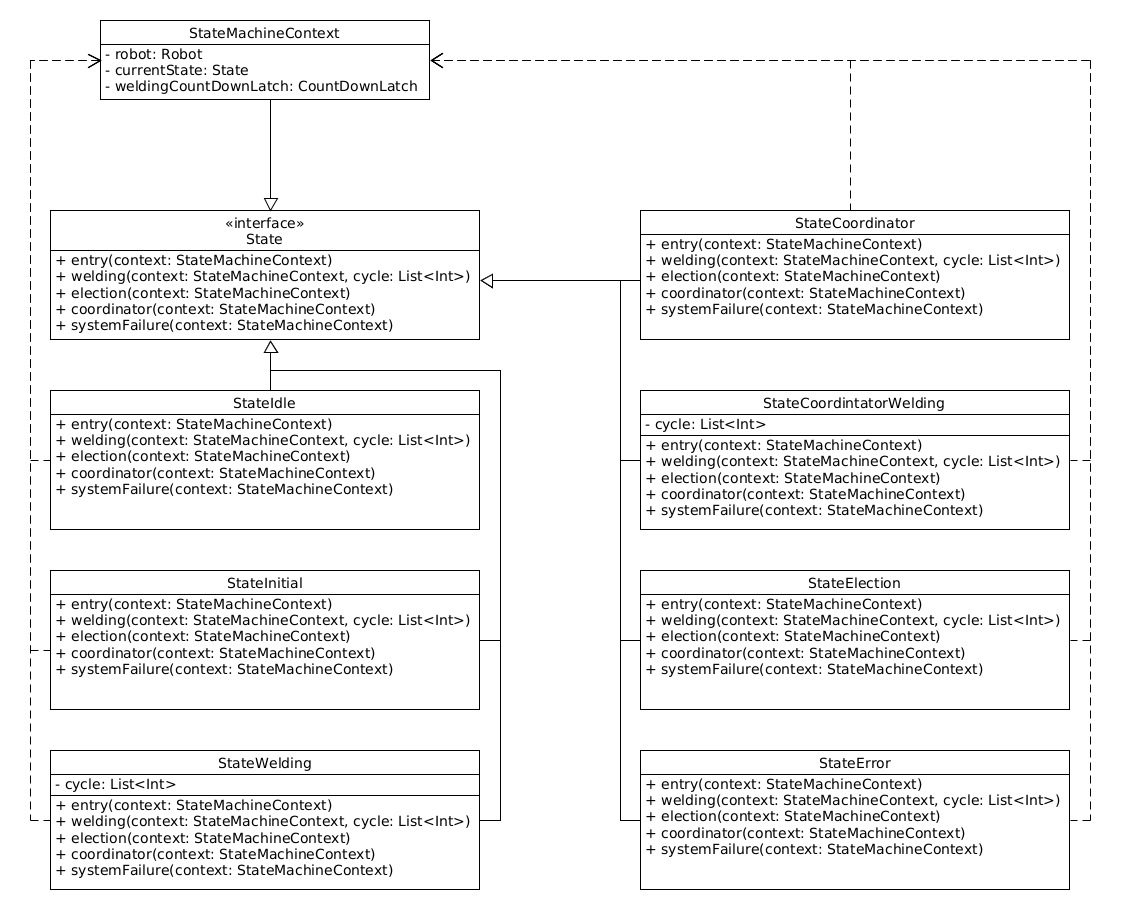
\includegraphics[width=\textwidth]{../diagrams/5_fsm_klassendiagramm.png}
 \caption{Klassendiagramm Statemachine}
 \label{fig:class_fsm}
\end{figure}

In Diagramm \ref{fig:class_fsm} ist das Klassendiagramm der FSM abgebildet. Für die Implementierung der FSM
wurde das State Pattern \citep{patterns} verwendet. Dieses ermöglicht eine übersichtliche und erweiterbare
Implementierung einer FSM, da jeder Zustand als Klasse implementiert ist und vom Interface \glqq State\grqq{}
(siehe \ref{fig:class_fsm}) erbt. Zum Hinzufügen von Zuständen muss eine neue Klasse implementiert werden, die 
von State erbt. Der StateMachineContext wird vom Roboter als Instanz gehalten und enthält zur Laufzeit immer
den aktuellen Zustand der FSM.

\clearpage

\subsection{Middleware}

\begin{figure}[h]
 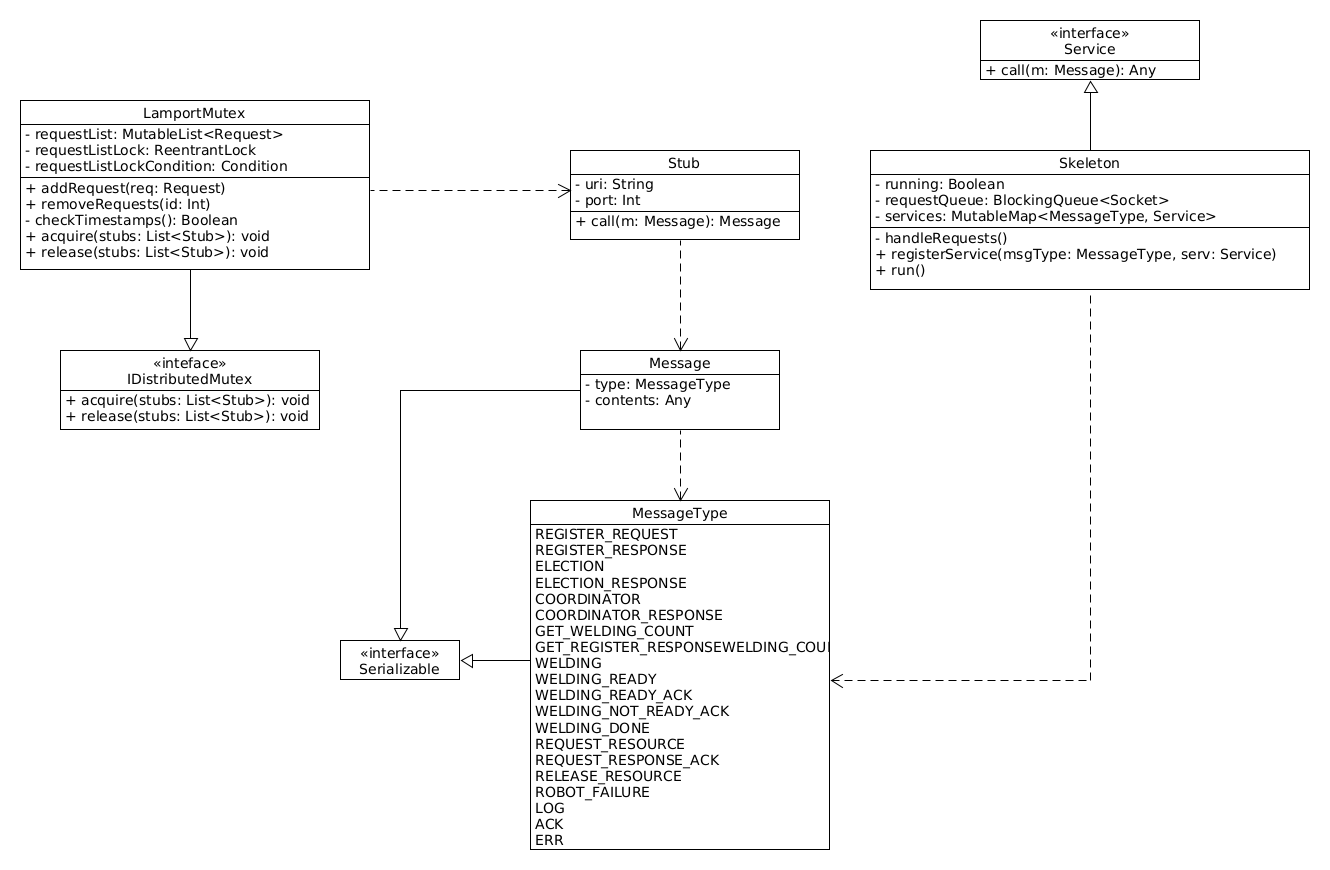
\includegraphics[width=\textwidth]{../diagrams/6_middleware_klassendiagramm.png}
 \caption{Klassendiagramm Middleware}
 \label{fig:class_middleware}
\end{figure}

Das Klassendiagramm \ref{fig:class_middleware} zeigt die Middleware mit RPC-Lösung. Stub und Skeleton arbeiten
mit Streams (ObjectInputStream \citep{objectinputstream}, ObjectOutputStream \citep{objectoutputstream})
zur Datenübertragung. Diese ermöglichen eine flexible RPC-Lösung, da auf ein externes 
Datenformat (z.B. json) für das Marshalling \citep{tanenbaumvansteen} verzichtet werden kann. Über die Streams lassen 
sich ganze Java-Objekte transferieren, in diesem Fall \glqq Message\grqq{} Objekte (siehe
\ref{fig:class_middleware}). Eine Message beinhaltet den MessageType und den eigentlichen Inhalt (Content) 
der Nachricht, worüber sich alle Dienste der RPC-Lösung abbilden lassen.

\clearpage

\section{Prozesse und Abläufe}

\subsection{StateMachine}

\begin{figure}[h]
 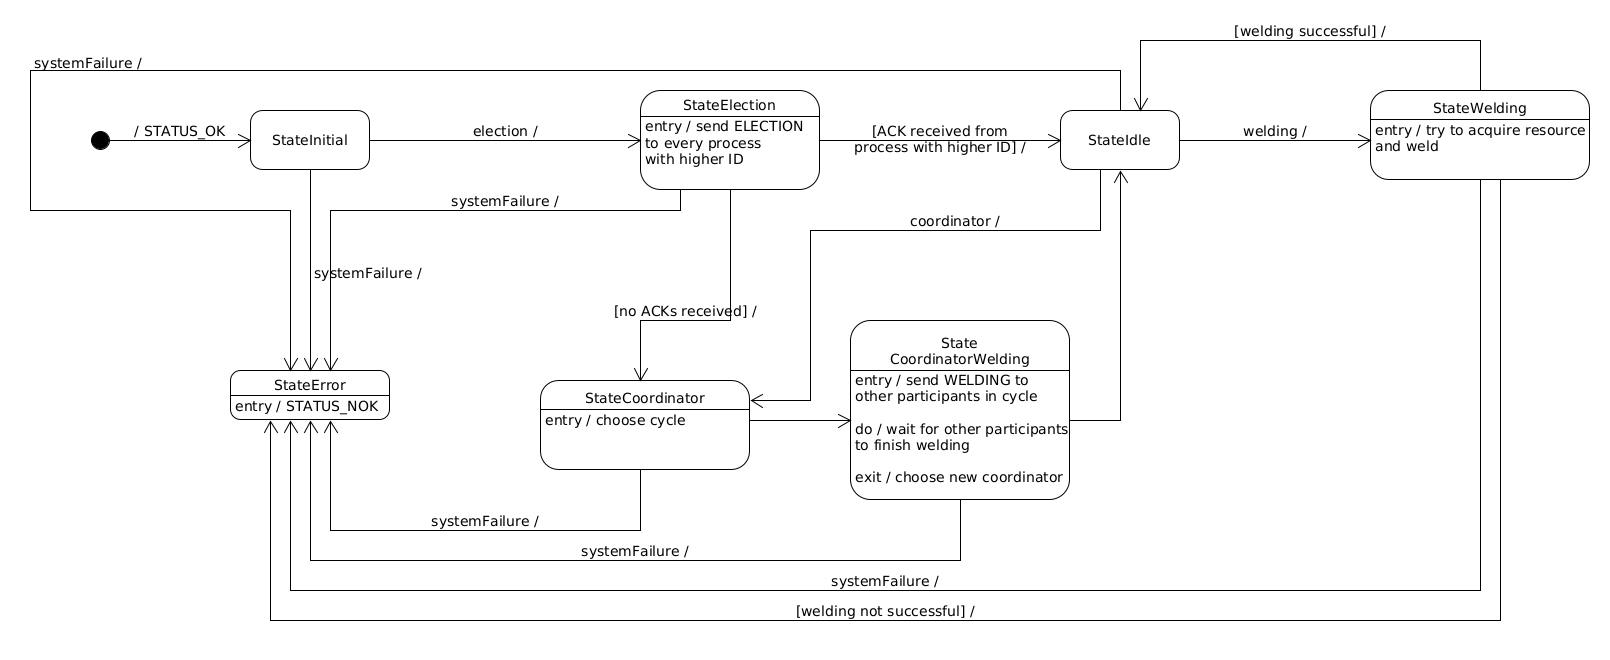
\includegraphics[width=\textwidth]{../diagrams/7_fsm.png}
 \caption{Zustandsdiagramm FSM}
 \label{fig:fsm}
\end{figure}

Die Statemachine, abgebildet in \ref{fig:fsm}, zeigt alle Zustände des Nodes und Roboters.
In den beiden States \glqq StateCoordinator\grqq{} und \glqq StateCoordinatorWelding\grqq{} ist die Logik
des Koordinators implementiert. Dadruch lassen sich Zyklen bestimmen und diese auch nacheinander ausführen.
Durch die Statemachine ist damit Anforderung \ref{table:reqchoosecycle} erfüllt.

\clearpage

\subsection{Registrierung}

\begin{figure}[h]
 \begin{center}
 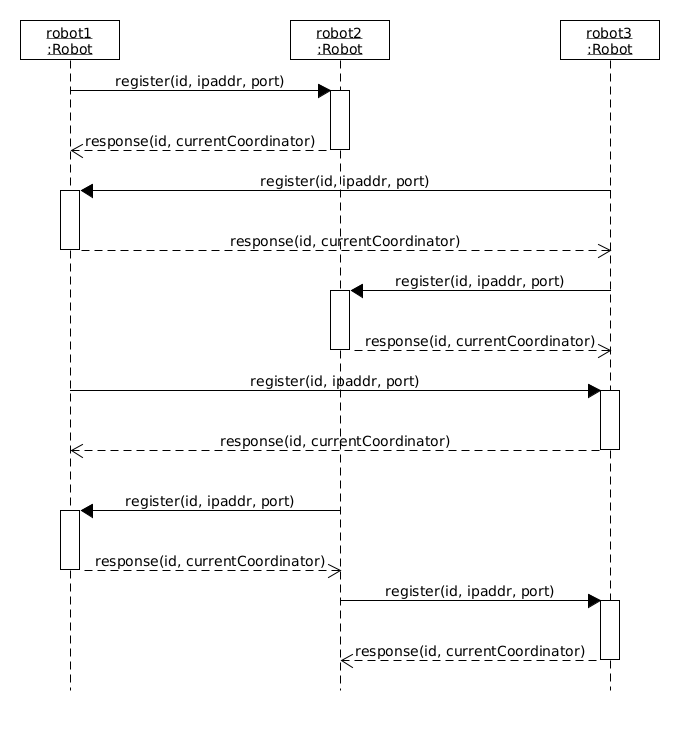
\includegraphics[width=0.7\textwidth]{../diagrams/8_sequence_register.png}
 \end{center}
 \caption{Sequenzdiagramm Registrierung}
 \label{fig:seq_reg}
\end{figure}

Im Sequenzdiagramm \ref{fig:seq_reg} ist der Registrierungsprozess von drei Robotern abgebildet.
Jeder Roboter schickt allen anderen in der definierten Portrange (siehe in Kapitel \ref{loesungsansatz}) einen
Registrierungsrequest mit seiner eigenen ID, seiner IP-Adresse und dem Port, auf dem er läuft.
Als Antwort erhält er die ID des Gegenübers und kann diese bei sich in der Teilnehmerliste eintragen.
Außerdem erhält er in der Antwort, falls bereits bestimmt, den aktuellen Koordinator im System. Wenn sich
ein Roboter später im System registriert, während zum Beispiel bereits ein Zyklus bearbeitet wird, trägt dieser
den aktuellen Koordinator bei sich ein und wartet bis er in einem Zyklus ausgewählt wird oder selber Koordinator
wird.

\clearpage

\subsection{Election}

\begin{figure}[h]
 \begin{center}
 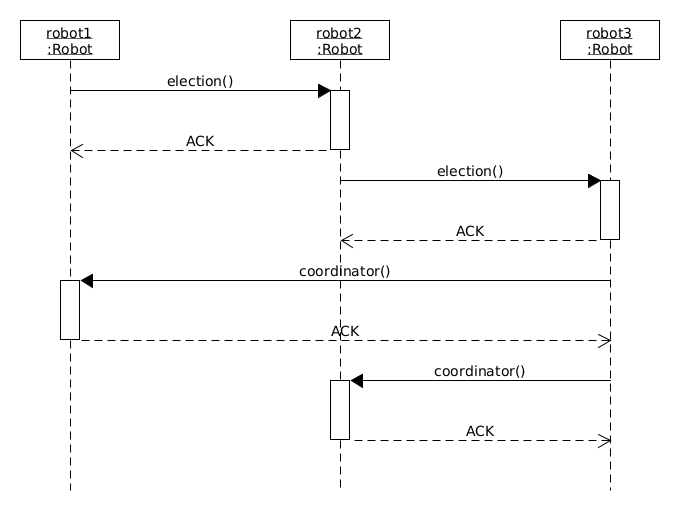
\includegraphics[width=0.8\textwidth]{../diagrams/9_sequence_election.png}
 \end{center}
 \caption{Sequenzdiagramm Election}
 \label{fig:seq_election}
\end{figure}

In Abbildung \ref{fig:seq_election} ist die Wahl des Koordinators mit dem Bully-Algorithmus abgebildet.
Wenn ein Experimentablauf gestartet wird und sich genug Roboter registriert haben, wird eine Wahl mit dem
Bully-Algorithmus angestoßen. Dadurch wird der erste Koordinator im System bestimmt, welcher einen Zyklus
auswählt.

\clearpage

\subsection{Schweißzyklus}

\begin{figure}[h]
 \begin{center}
 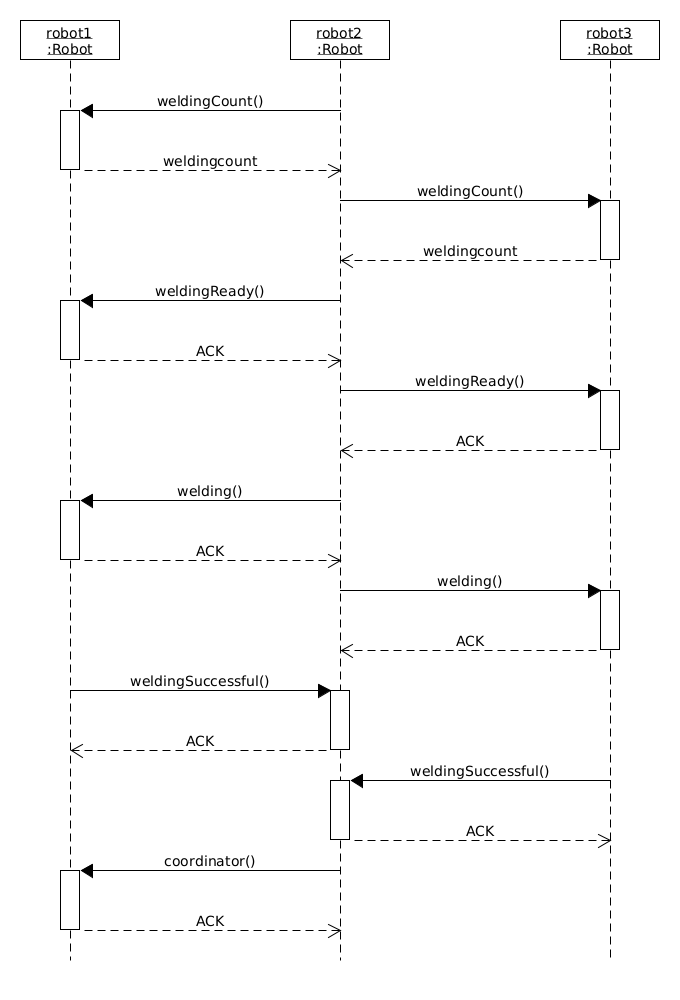
\includegraphics[width=0.49\textwidth]{../diagrams/10_sequence_welding.png}
 \end{center}
 \caption{Sequenzdiagramm Schweißzyklus}
 \label{fig:seq_welding}
\end{figure}

Das Sequenzdiagramm \ref{fig:seq_welding} zeigt einen Schweißzyklus mit drei Robotern. Roboter Nr. 2 (robot2)
ist der aktuell ausgewählte Koordinator.
Zunächst holt der Koordinator sich die Anzahl abgeschlossenen Schweißaufträge aller anderen Roboter im System
um zu bestimmen, welche Roboter im Zyklus schweißen sollen. Die zwei Roboter mit der niedrigsten Zahl
an abgeschlossenen Schweißaufträgen werden als Teilnehmer im Zyklus gewählt. Dadurch wird sichergestellt,
dass kein Roboter mehr als drei Mal so oft geschweißt hat wie ein anderer im System (siehe Anforderung
\ref{table:reqprocess}).
 Wenn dies geschehen ist, wird gefragt ob alle Teilnehmer des Zyklus bereit zum schweißen sind. 
Wenn alle Teilnehmer ihre Bereitschaft bestätigt haben, gibt der Koordinator den anderen Robotern
und sich selbst die Anweisung zu schweißen. Die Reihenfolge der Schweißvorgänge wird durch den 
Lamport-Algorithmus festgelegt. Während des Schweißvorgangs wird parallel die Zykluszeit vom 
Koordinator überwacht, sollte diese überschritten werden, wird das System in einen Fehlerzustand 
versetzt (siehe UseCase \ref{table:usecase1}).

\clearpage

\subsection{Roboterausfall}

\begin{figure}[h]
 \begin{center}
 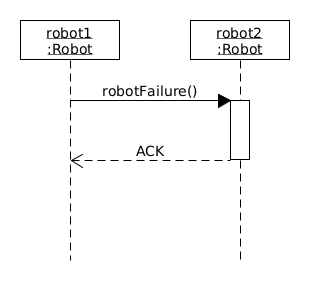
\includegraphics[scale=1]{../diagrams/11_sequence_robot_fail.png}
 \end{center}
 \caption{Sequenzdiagramm Roboterausfall}
 \label{fig:seq_failure}
\end{figure}

Wenn ein Roboter nach einem Schweißauftrag in einen Fehlerzustand wechselt, sendet er an alle anderen
Teilnehmer eine Nachricht, dass der Roboter nicht mehr betriebsbereit ist (siehe \ref{fig:seq_failure}).
Die Roboter, die diese Nachricht erhalten haben löschen den Roboter aus ihrer Teilnehmerliste und wird
für den weiteren Experimentverlauf nicht mehr berücksichtigt.
